\part{Introduction}
\section{Preface}
Thanks to the rapid development of experimental techniques at the cellular level, over the last century there was a tremendous progress in the fields of human physiology, immunology and therapeutics. The breakthrough discoveries were based mainly on the analysis of biochemistry (either intercellular or intracellular molecular pathways).
Mechanical properties of investigated objects were often either completely neglected, or strongly underestimated. However, all living cells are exposed to the action of external forces: fluid-mediated (eg. blood flow) or structure-mediated (eg. body weight strain in bones). The process of converting external mechanical stimuli into biochemical signals (and in turn into physiological responses) is called mechanotransduction. 
\newline 
The most appealing discovery, which evidences for the importance of mechanical properties, refers to the fate of stem cells. In 2006 Engler \emph{et al.} identified a new factor capable to regulate the fate of stem cells: the elasticity of the microenvironment (matrix). Namely, by changing the elastic properties of the substrate, stem cells could be directed towards muscle, bone or even neuronal lineages \cite{Even-Ram2006}. On the grounds of the recent discoveries, the new field of science have emerged: \emph{mechanobiology}. It is targeted to study the mechanotransduction processes at the level of tissues and cells, and the way it influences the development, physiology and diseases.
One may wonder what is the range of forces capable to elicit a cellular response. It is reasonable to assume, that the effect of force should exceed the energy of thermal fluctuations. At $37\degree C$ the thermal energy, $kT$, is about $4\;pN\cdot nm$. Considering the conformational changes in peptide-based molecular transducers have a characteristic length scale within the range of $1 - 10\;nm$, then it would correspond to the force of $0.4-4\;pN$. Interestingly, Finner \emph{et al.} (1994) have estimated, that a single myosin molecule, which drives contractility action and thus can induce cell signaling, is capable to produce a force $3-4\;pN$ \cite{Silberberg2008}. Therefore, it turns out that mechanotransduction is induced by forces only slightly higher than thermal fluctuations, \emph{i.e.} within the range of $10^0-10^1$ piconewtons. Obviously, the sensitivity and concentration of force transducers strongly depends on the type of cell and its location in human body.
\newline

The endothelium is formed by the monolayer of cells lining the lumen of all blood vessels in human body. \Glspl{EC} serve as a barrier between blood and the rest of the system. Thus, their physiology is affected by numerous biochemical factors. The dysfunction of endothelium contributes to the development of numerous systemic civilization-wide diseases, \emph{inter alia} hypertension, atherosclerosis and diabetes. Therefore, a deep understanding of its functioning is one of the main interest in terms of the development of proper treatments. The vascular system is a highly dynamic structure, with component-rich blood constantly circulating in the pace of heart beats, which is followed by vessel vasodynamics. Moreover, it provides highly versatile environments -- human circulatory system is over 100 000 000 meters long and the luminal diameter varies from several centimeters (\emph{eg.} aorta) to submilimeter values (mirovessels) \cite{Loe2004, Fu2013}. Therefore, a great input to cardiovascular physiology is provided by mechanobiology of endothelium, which in turn may be considered in terms of two classes: cell mechanics and external mechanical stimuli \cite{Fels2014}. The extracellular stimulation is exerted by the cell-cell contacts and the blood flow (shear stress, circumferential stretch and hydrostatic pressure). Complementary, endothelial (nano)mechanics is understood in terms of mechanical properties of cellular structures and their variations triggered either by intracellular processes or external stimuli. Considering the importance of endothelial physiology for the homeostasis of human body and the particular role that is played by \glspl{EC} nanomechanics, these type of cells became a primary focus in the presented work.

Only recently, mechanical properties of endothelial cellular structures were proven to be in correlation with intracellular biochemical processes. The studies presented in literature mostly relate cortical elasticity variations to the changes of selected biochemical factor. 
Attempts employing various experimental techniques have been made, involving optical tweezers \cite{Wang2006, Hayakawa2008}, magnetic bead pulling/twisting \cite{Bausch2001, Zeng2010} and pipette aspiration \cite{Sato1987, Zeng2011}. 
However, the most prominent advances in this area have been made using \gls{AFM}. The group of Oberleithner (University of M\"{u}nster, Germany) became a leader in studying endothelial nanomechanics. Using nanoindentation spectroscopy with an \gls{AFM} tip, they have connected elasticity changes with aldosterone treatment \cite{Oberleithner2005}, sodium \cite{Oberleithner2007a} and potassium \cite{Oberleithner2009} concentration, \gls{NO} production \cite{Fels2010_trois}, C-reactive protein \cite{Kusche-Vihrog2011} and \gls{ENaC} activity \cite{Kusche-Vihrog2008}. Using the same technique, our group have described the alterations of \glspl{EC} mechanical properties during the development of inflammatory state triggered by \gls{TNF} \cite{Szczygiel2011}, as well as during the anti-inflammatory action of 1-methylonicotinamid chloride \cite{Kolodziejczyk2013}. Moreover, we have discovered the stiffness memory of \glspl{EC} in response to chronic hyperglycemia \cite{Targosz-Korecka2013}. 
The presented \gls{AFM}-based investigations considered the \gls{AFM} probe-cell mechanical interaction in terms of simple elastic (Hertzian) deformation. Thus, the \gls{EC} mechanical properties were effectively determined by elasticity of cell cortex (mainly cortical actin skeleton). As there exist numerous cell structures relevant in terms of nanomechanics (see section \ref{sec:cellular_structures}), lately this simplified approach became a matter of discussion. As a result, last year two papers presenting either only mechanical properties of \gls{eGC} \cite{Wiesinger2013} or \gls{eGC} together with cortical elasticity has been published. However, the presented methodology is still to be improved in order to obtain objective, unbiased results.

The presented dissertation focuses on the development of experimental protocols and data analysis procedures targeted to differentiate nanomechanical properties of individual structures in \glspl{EC}. The study was aimed at the in vitro cultured \glspl{EC} whose mechanics has been assessed basing on the character of interaction during nanoindentation with a tip of \gls{AFM}. The work is organized in the following way. Firstly, the models of interactions occuring during cell indentation with a probe will be introduced. Next, the nanoindentation data are analysed separately during probe approach, relaxation (pause segment) and retraction. Each of these segments is used to resolve information about individual cellular structures, namely \gls{eGC}, cell membrane, cell cortex and bulk. In addition, a tip-induced mechanotransduction effect is presented in section XX. Lastly, section XX describes the research, where solid-state \gls{AFM} probe has been replaced by a living \gls{EC}, which then was used to probe cell-cell interaction. The proposed experimental methodology provides solid foundations to use alterations in cell structures nanomechanics as a sensitive bioindicator of the physiological state of endothelium. 


This work was supported by the European Union from the resources of the European Regional Development Fund under the Innovative Economy Programme (grant coordinated by JCET-UJ, No POIG.01.01.02-00- 69/09). Part of this project (tip-induced mechanotransduction) has been also supported by the grant of the Polish Ministry of Science and Higher Education number 7150/E-338/M/2013.


\section{Cellular structures determining mechanical properties of cells}\label{sec:cellular_structures}
Animal cell is a complex living biological machinery containing nucleus and other membrane-bound organelles (mitochondria, Golgi aparatus etc.) suspended in cytosol. The presented description will apply to \gls{EC}, however a significant part of the facts hold for other human cell types. \Glspl{EC} form a tight monolayer on the luminal part of vessels, which permeability is mostly gated by those cells. Cells are highly sensitive to deformation. In the first approximation, they may be considered as a membrane-limited container filled with incompressible fluid (cytosol). Therefore, the application of an external force results in mechanical deformation of the surface, which causes the displacement of the fluid. In order to counteract the susceptibility to such stimuli and stabilize the shape, cells have developed a multilevel system of cytoskeletal structures, namely: actin filaments, intermediate filaments and microtubules. Moreover, the cellular membrane is decorated with glycan-rich brush referred to as \gls{eGC}.


\begin{figure}[tb]%H
\centering
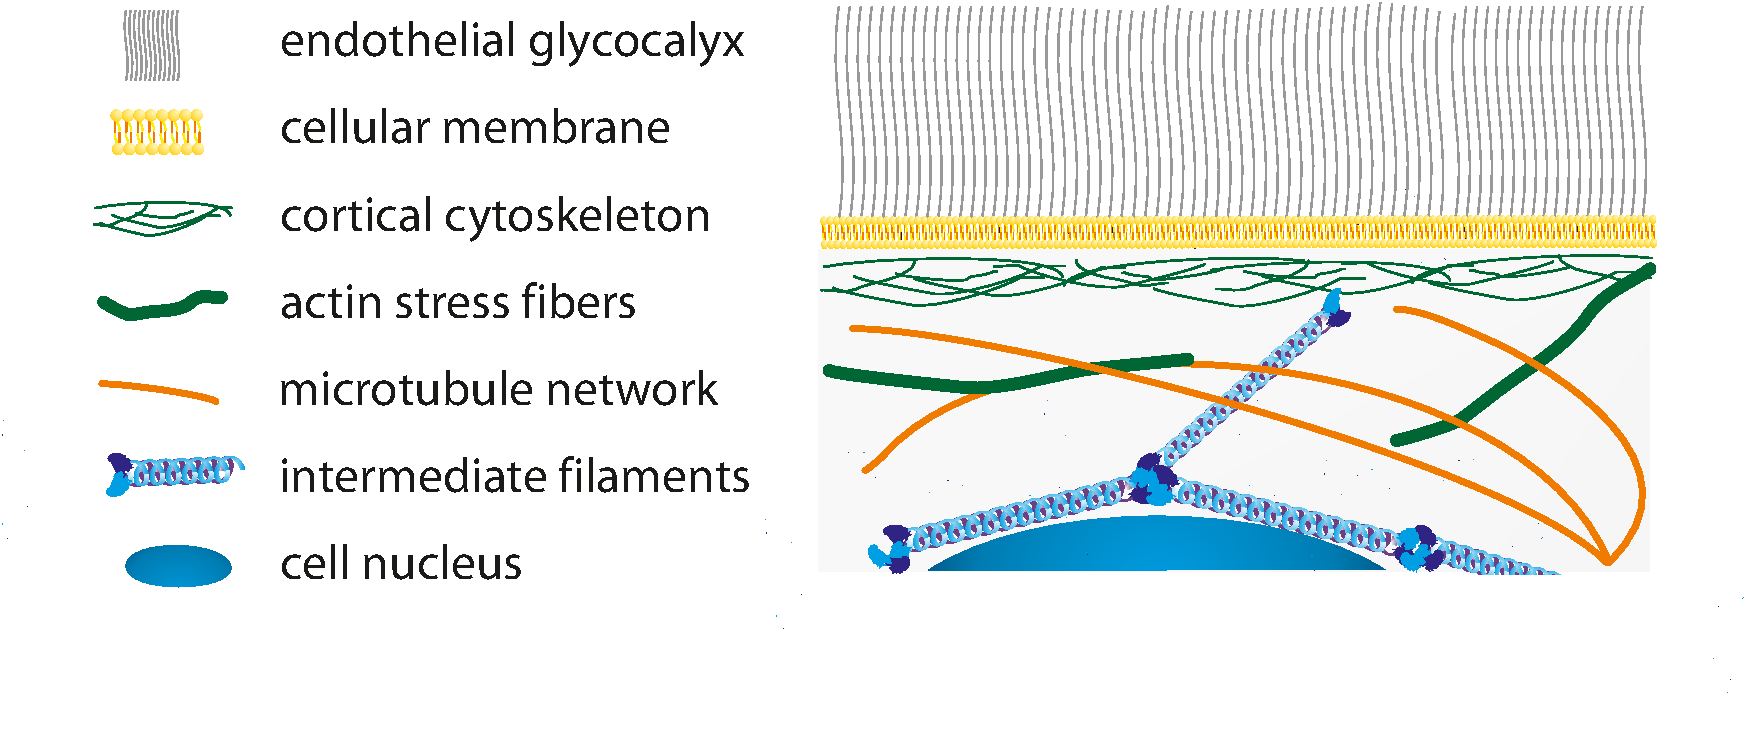
\includegraphics[width=0.9\textwidth]{schemat_komorki.pdf}
\caption[Scheme presenting cellular structures determining mechanical properties of \gls{EC}.]{The drawing presents cell components, which determine mechanical properties of \gls{EC}. The details of the structure composition and functions are presented in the text. Please note the elements are not in scale.}
\label{fig:intro:cell_structure}
\end{figure}
The schematic drawing of cell presenting the composition of cellular structures meaningful in terms of cellular mechanics is presented in Figure \ref{fig:intro:cell_structure}. Below, we will provide a brief description of each structure and its function.
\begin{description}
\item[endothelial glycocalyx] It decorates the luminal surface of \glspl{EC} monolayer. \glspl{eGC} is composed of various proteoglycans, glycosaminoglycans and plasma proteins.
\item[cellular membrane]
\item[cortical cytoskeleton]
\item[actin stress fibers]
\item[microtubule network]
\item[intermediate filaments]
\item[cell nucleus]
\end{description}